\documentclass{standalone}
\usepackage{tikz}
\usepackage{calc}
\usepackage{bm}
\usepackage{graphicx}
\usepackage{amsmath}
\usetikzlibrary{calc,shapes,shapes.geometric, arrows, fit}
\pgfdeclarelayer{background}
\pgfdeclarelayer{foreground}
\pgfsetlayers{background,main,foreground}
\makeatletter
\begin{document}

\tikzstyle{decision} = [diamond, draw, fill=blue!20,
    text width=4.5em, text badly centered, node distance=3cm, inner sep=0pt]
\tikzstyle{block} = [rectangle, draw, fill=blue!20,
    text width=6em, text centered, rounded corners, minimum height=4em]
\tikzstyle{block2} = [rectangle, draw, fill=red!20,
    text width=6em, text centered, rounded corners, minimum height=4em]
\tikzstyle{line} = [draw, -latex]

\begin{tikzpicture}[node distance = 2cm, auto]
    % Place nodes
    \node [block] (init) {Inicialización};
    \node [block, below of=init] (camara) {Recoger imagen de la cámara};
    \node [block, below of=camara] (marcadores) {Detectar marcadores};
    \node [decision, below of=marcadores] (decide) {\footnotesize ¿Hay algún marcador?};
    \node [block, below of=decide, node distance=3cm] (posicion) {Estimación de la posición};
    \node [decision, below of=posicion] (decide2) {\footnotesize ¿Posición válida?};
    \node [block, below of=decide2, node distance=3cm] (inversion) {Inversion de posición y orientacion};
    \node [block, below of=inversion] (envio) {Envio al autopiloto};

    % Draw edges
    \path [line] (init) -- (camara);
    \path [line] (camara) -- (marcadores);
    \path [line] (marcadores) -- (decide);
    \path [line] (decide) -| node [near start] {no} ++(-3,3) coordinate (aux1) |- (camara);
    \path [line] (decide) -- node {sí}(posicion);
    \path [line] (posicion) -- (decide2);
    \path [line] (decide2) -| node [near start] {no} ++(3,3) coordinate (aux2) |- (camara);
    \path [line] (decide2) -- node {sí}(inversion);
    \path [line] (inversion) -- (envio);
    \path [line] (envio) -| node [near start] {} ++(-3,3) |- (camara);

    \path (-1,2.5) node(cam)[inner sep=-1cm]{\includegraphics[width=1cm]{camera.png}};
    \path (1,2.5) node(rpi)[inner sep=-1cm]{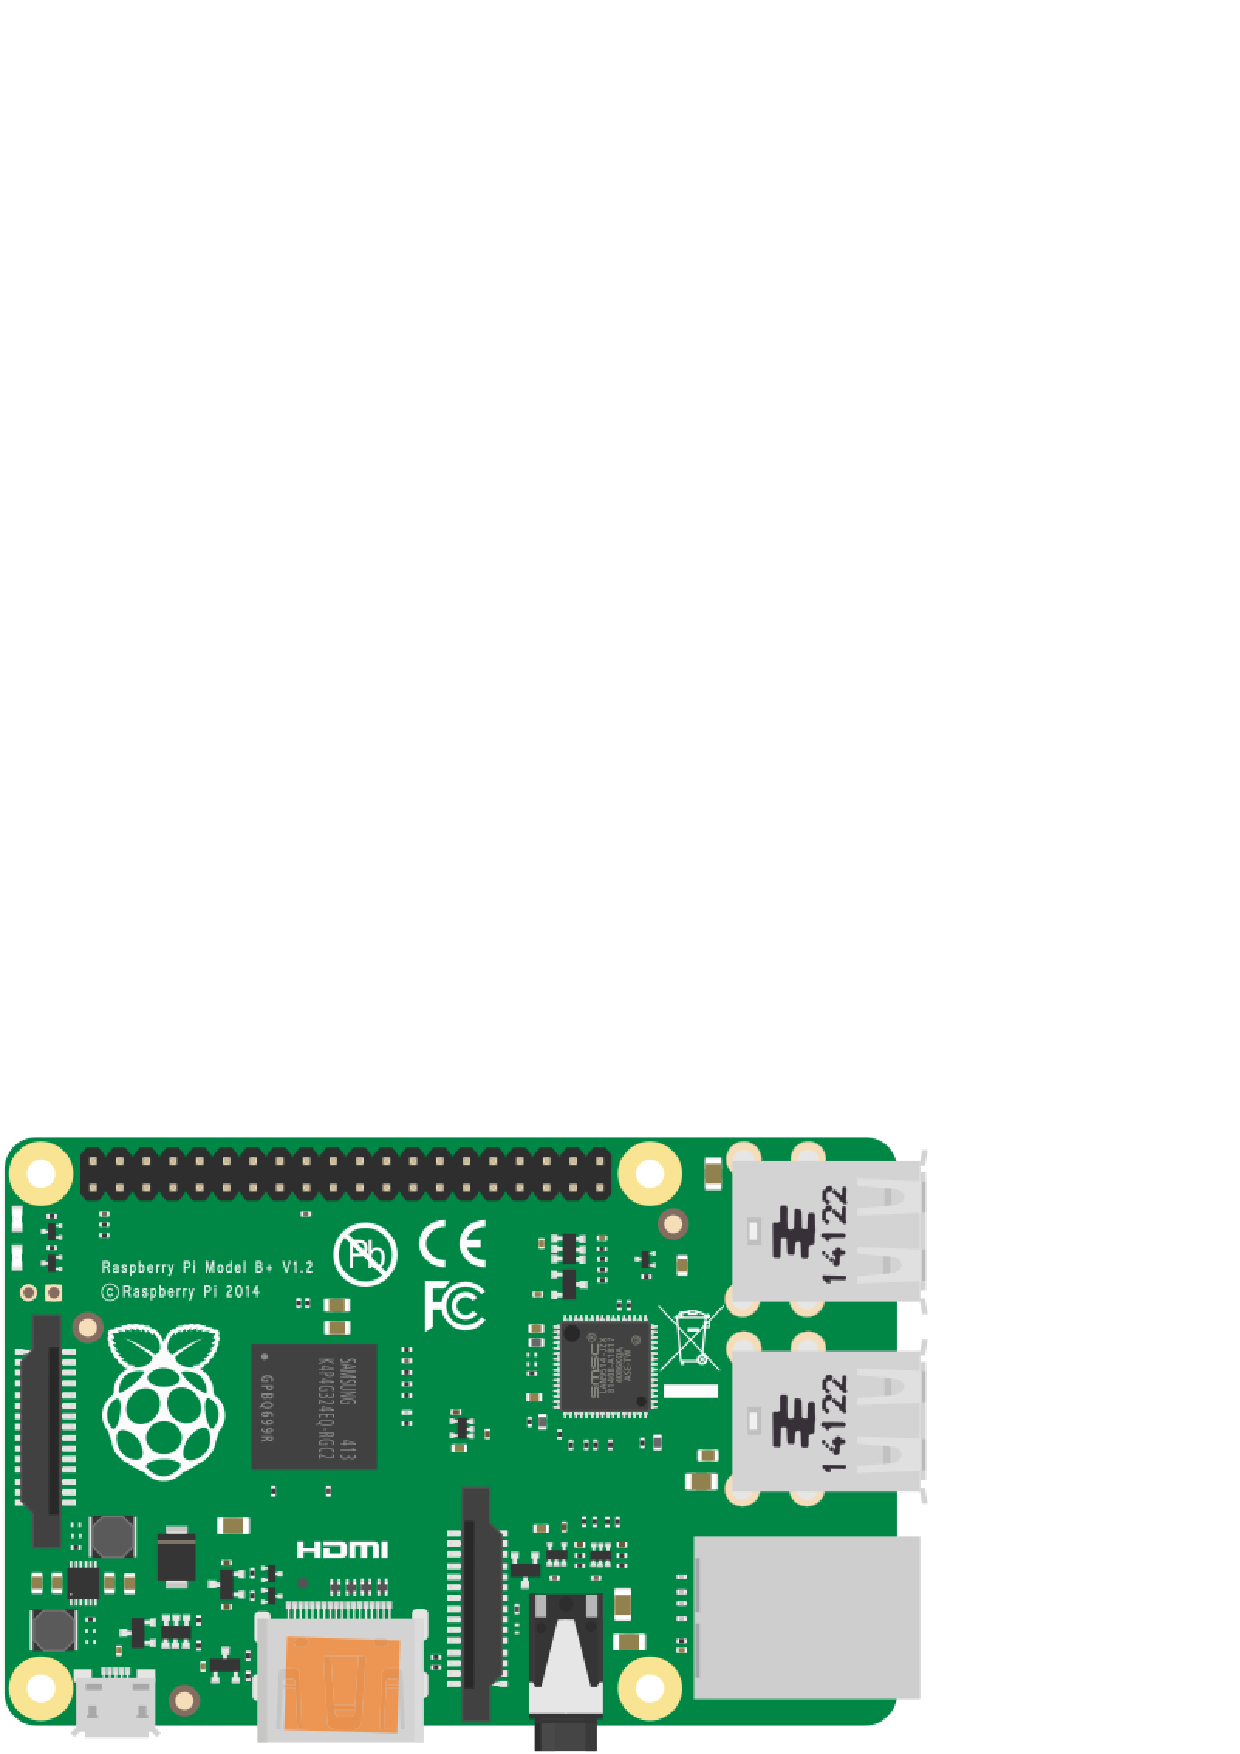
\includegraphics[width=2.5cm]{raspberry.pdf}};

    \begin{pgfonlayer}{background}
        \path node(box1)[fit=(init) (envio) (aux2) (aux1) (cam) (rpi),draw, inner sep=1cm, rounded corners, fill=yellow!20]{};
    \end{pgfonlayer}

    % Autopiloto

    \path (box1.east) ++ (8,0) node(EKF)[block]{Estimador de estados};
    \path node(control)[block, below of=EKF]{Control de posición y velocidad};
    \path node(orientacion)[block, below of=control]{Control de orientación};

    \path [line] (EKF) -- (control);
    \path [line] (control) -- (orientacion);
    \path [line] (EKF.east) -- ++ (0.5,0) |- (orientacion);

    \path (EKF) ++ (0,2.5) node[ inner sep=-1cm](cuav){\includegraphics[width=2.5cm]{cuav.png}};
    

    \begin{pgfonlayer}{background}
        \path node(box2)[fit=(EKF) (cuav) (control) (orientacion),draw, inner sep=1cm, rounded corners, fill=red!10]{};
    \end{pgfonlayer}

    \draw (box1.east) edge[bend left=30,-latex] node[anchor=south, align=center]{\Large  $\bm{p}$, $\Psi^{Marcador\rightarrow UAV}$} (EKF.west) ;

\end{tikzpicture}

\end{document}
